\documentclass[9pt]{extarticle}
\usepackage[english]{babel}
\usepackage[plain]{fullpage}

\usepackage{multicol}
\usepackage[dvipsnames]{xcolor}
\usepackage{graphicx}
\graphicspath{ {images/} }

\usepackage{hyperref}
\hypersetup{
  colorlinks=true,
  linkcolor=BrickRed,
  % citecolor=BrickRed,
  urlcolor=BrickRed
}

\title{Information Retrieval \\ \textsc{Project}}
\author{Krikun Gosha, Arthur Korochansky, Roman Sotnichenko}
\date{}

\begin{document}

\maketitle
\paragraph*{Distributed crawler framework} with extendable layers.\\

\subsection*{Preface}
\begin{multicols}{2}
In this project we should engineer system with crawling functionality on cluster
of commodity hardware\footnote{commodity hardware --- computers that we can see at
home, work, office}. All requests to network resource completes from each
machine by themselves, but from addresses, given by master task scheduler.

Replies stores in the machine memory (preferably at RAM with disc's
replications). Each machine reports to master its status (stored blocks, load
status etc.) and provide ability to manage data and execute computations closely
to data. 

Master could produce response on users requests, queries. It could be text
search or other computations. But it could be a case when replies are sent by
required computers at cluster.\\

Also we should mention connection interface and different connection schemes in
networks:\\

\begin{center}
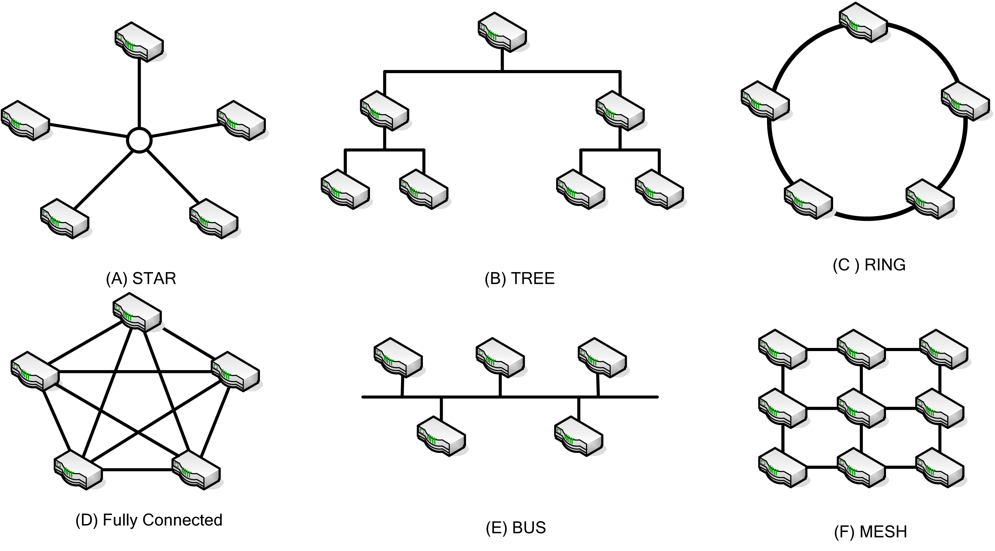
\includegraphics[width=0.9\linewidth]{connections}

{\footnotesize                  
and all possible derived graphs 
}
\vfill

But let's not go into too much details too soon.
\end{center}


\columnbreak

Return to our crawler. Primary functionality is creation image of a network for
performing some kind of distributed computations in short time.   

Therefore it should be implement as kind of layer and be able to determine the
network structure somehow, parse structure and provide task manager for running
useful staff. 

For determining network structure we have to parse pages' links. Or if we
have DNS data, we can make direct access and then search through pages links...\\ 

{\footnotesize
By the way about DNS routing. Each server keeps tables in L1-L2 caches to
respond as quickly as possible. This is quite good example to observe,
\textit{the fastest memory closer, more expensive, smaller.}
}\\

We present the network as a graph, thus we could build link graph, index anchor
text. That functionality should be consider with master task scheduler (aka
JobTracker), which delegate work by chunks to slave nodes.
Obviously they have common functionality.\\

But in the end we should fetch whole network's pages. And preferably limit load
on crawled servers (respect robots.txt, be polite, don't lie).\\


% Thus, by access to crawl data, after what, we could respond to user requests.
Firstly lets consider open-source solutions

\begin{itemize}
\item{
    Apache Nutch
  }
\item{
    Hadoop Ecosystem
  }
\item{
    In-memory Computing Platforms
  }
\item{
    Distributed Programming
  }
\end{itemize}

\end{multicols}


\vfill
\pagebreak

\subsection*{Open source solutions}

\begin{multicols}{2}
% \section{Apache Nutch}
\textbf{Apache Nutch} is distributed crawler framework with extendable layers.

In first version it uses Hadoop framework (actually starts as a part of crawler)
and other open source solutions for crawling on different machines, storing
information separately on each of them and providing possibility to execute
operations and computations of this information directly on it.\\

\columnbreak

\textbf{Hadoop} is environment write in Java for creation computational cluster.

Based on two basic layers (could be extensible):

- Hadoop Distributed File System (HDFS)

- MapReduce computational strategy

Actually Hadoop ecosystem contains a lot of additional software packages for
different kind of functionality (eg. Hive, Pig, YARN, Ignite, Spark etc).  



% basically on cluster of
% commodity hardware.   
\end{multicols}

\begin{center}
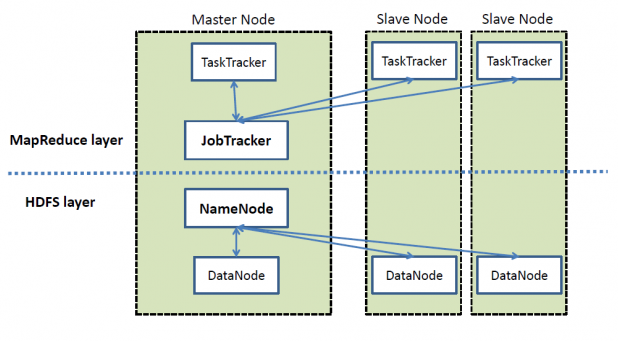
\includegraphics[width=0.6\linewidth]{hadoop}
\end{center}

\begin{multicols}{2}

\textbf{HDFS layer}
stores data in chunks, divided on several machines and providing basic access
operations. 

Master Node knows on which Slave Node located needed block of information.
Overall it represents access point to distributed file system. 

\columnbreak

\textbf{MapReduce layer}
provides us ability to execute work directly on machine with data and get
results back. Lately we could apply reduction on results, set of separate
computations (eg. amount words in blocks). 

It is good strategy if work could divide in pieces.
\end{multicols}

This gives to us possibility to scale system horizontally, adding more machines
into the cluster.  

% In second Apache Gora (in which many ideas are derived from Hadoop).

And consider Hadoop ecosystem we can generalize approach like GridGain\footnote{
  GridGain is open source project licensed under Apache 2.0. One of the main
  pieces of this platform is the In-Memory Apache Hadoop Accelerator which aims
  to accelerate HDFS and Map/Reduce by bringing both, data and computations into
  RAM. This work is done with the GGFS - Hadoop compliant in-memory file
  system.}
did: 

% For I/O intensive jobs GridGain GGFS offers performance close to 100x
% faster than standard HDFS. Paraphrasing Dmitriy Setrakyan from GridGain Systems
% talking about GGFS regarding Tachyon: 

%     GGFS allows read-through and write-through to/from underlying HDFS or any
%     other Hadoop compliant file system with zero code change. Essentially GGFS
%     entirely removes ETL step from integration. 

%     GGFS has ability to pick and choose what folders stay in memory, what
%     folders stay on disc, and what folders get synchronized with underlying
%     (HD)FS either synchronously or asynchronously. 

%     GridGain is working on adding native MapReduce component which will provide
%     native complete Hadoop integration without changes in API, like Spark
%     currently forces you to do. Essentially GridGain MR+GGFS will allow to bring
%     Hadoop completely or partially in-memory in Plug-n-Play fashion without any
%     API changes. 

\begin{center}
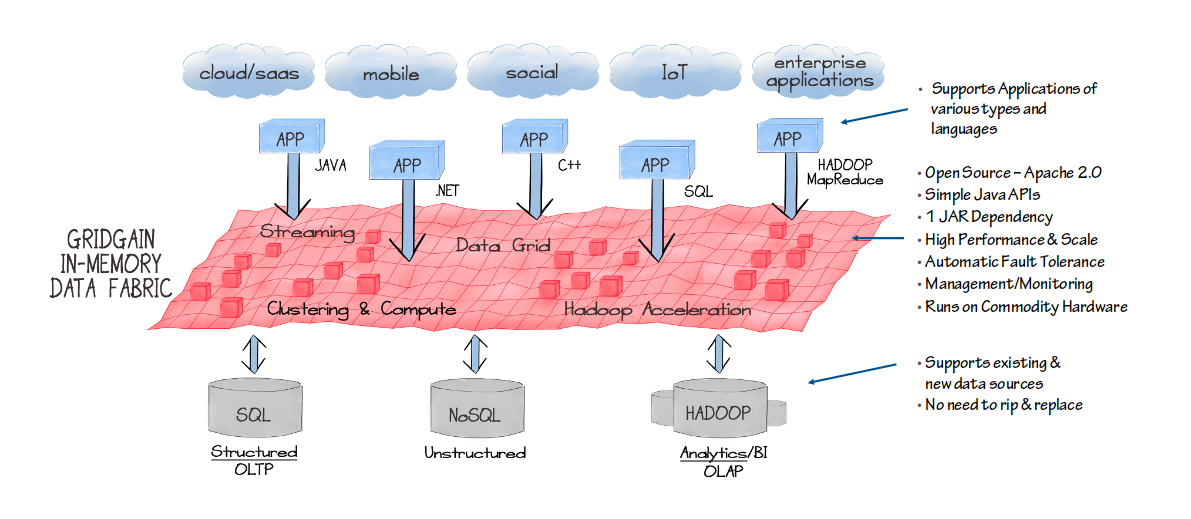
\includegraphics[width=\linewidth]{approach}
\end{center}

\vfill

\bibliographystyle{unsrt}
\bibliography{report}


\end{document}